\documentclass[12pt]{article}
 
\usepackage[margin=1in]{geometry} 
\usepackage{amsmath,amsthm,amssymb}
\usepackage[lofdepth,lotdepth]{subfig}
\usepackage{float}
\usepackage{graphicx}
\usepackage{float}
\usepackage{tikz}
\usepackage{caption}
\usetikzlibrary{arrows,shapes,trees} % loads some tikz extensions
 
\begin{document}
\graphicspath{{images/}}
 
\title{CSE 802 - Final Project Report\\ ImageNet Classification}
\author{Sunpreet Arora \& Josh Klontz\\
}
 
\maketitle

\section{Introduction}
Automated image classification is a classic problem in the domain of computer vision and pattern recognition.
Although numerous algorithms exist for categorizing images based on their distinct features, large scale image classification is still considered an open problem.
This is primarily because as the number of classes increases, it becomes increasingly difficult to find a distinctive set of features to distinguish between them.
Compounding the problem, the computational complexity of the classification task generally scales with the number of classes.

Arguably the most common approach to image classification is the popular information retrieval model known as the bag-of-words (BOW) model.
A \textit{visual vocabulary} is first created based on features computed from the training set.
Images are then represented and classified based on the frequency of occurrence of their features (also referred to as \textit{visual words}) in the visual vocabulary.

Several databases have been collected to advance the state-of-the-art in image classification including Caltech 101 \cite{caltech101}, and PASCAL VOC \cite{pascal09}.
ImageNet \cite{imagenet} is one of the most recent large scale image databases with 10,000 image classes, and over a million images.
Convolutional neural networks (CNNs) have been reported to give the best rank-5 accuracy of around 85\% on the ImageNet database \cite{alex2012}.
However, they were implemented on massively parallel GPU's.
Another effective approach with a reported top-5 accuracy of 74\% involves Fisher vectors \cite{csurka2011fisher}.

The scope of this project is limited to classifying a subset of 20 classes (the 10 hardest and 10 easiest) from the ImageNet database.
We are given about 20000 images for training, 1000 images for validation and 5000 images for testing.
The objective is to come up with a classification framework that maximizes rank-5 accuracy.

\section{Challenges}
Despite working on a 20 class subset of ImageNet, the classification problem is still very challenging.
Some of the most challenging aspects are briefly discussed below.

\begin{itemize}
\item \textit{Intraclass Variability}:
Since ImageNet database is organized in a semantic hierarchy, exemplars from the same image class exhibit a considerable amount of variation or \textit{intraclass variability} amongst themselves.
For example, both a gong and a wind chime belong to the semantic category (Figure \ref{fig1:intraclassvariability}).

\item \textit{Interclass Similarity}:
Similarly, exemplars from different classes such as spatula and ladle look visually similar to each other, or in other words exhibit \textit{interclass similarity} (Figure \ref{fig1:interclasssimilarity}).

\item \textit{Scale}:
The object of interest is present at different scales in different exemplar images for two canoe images (Figure \ref{fig1:scale}).

\item \textit{Occlusion}: Sometimes the object of interest is occluded by another object in the image, thereby reducing the amount of useful information content for the classification task like the drill and the spatula (Figure \ref{fig1:occlusion}).

\item \textit{Pose}:
Variations in pose of the object of interest are also observed amongst different exemplar images. The hatchets in this example face different directions (Figure \ref{fig1:pose}).

\item \textit{Illumination}:
The database contains images acquired from a lot of different sources with differing illumination conditions, like the cleavers shown below (Figure \ref{fig1:illumination}).

\item \textit{Clutter}: There is a lot of background clutter in some of the exemplar images, or in other words there is more useless or distracting information present in the image than the useful signal for the purpose of image classification (Figure \ref{fig1:clutter}).
The correct classes in this example are cleaver and spatula.

\end{itemize}

\begin{figure}
\centering
\subfloat[intraclass variability]{
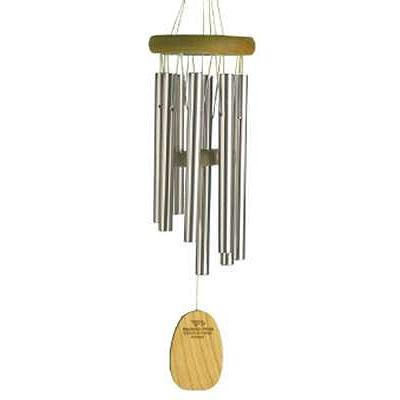
\includegraphics[width = 0.2\textwidth, height = 0.15\textheight]{chime1}
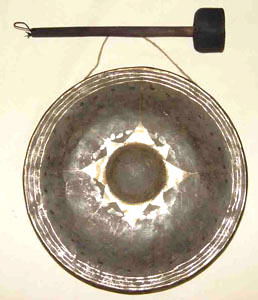
\includegraphics[width = 0.2\textwidth, height = 0.15\textheight]{chime2}
\label{fig1:intraclassvariability}
}
\subfloat[interclass similarity]{
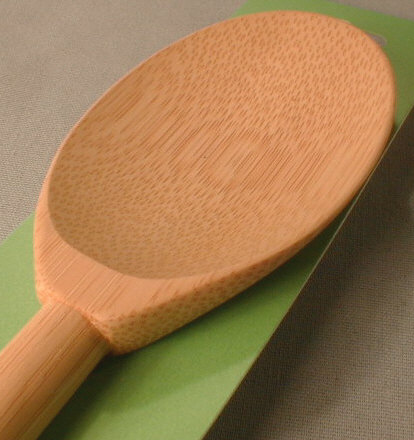
\includegraphics[width = 0.2\textwidth, height = 0.15\textheight]{spatula1}
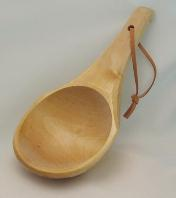
\includegraphics[width = 0.2\textwidth, height = 0.15\textheight]{ladle1}
\label{fig1:interclasssimilarity}
}
\qquad
\subfloat[scale]{
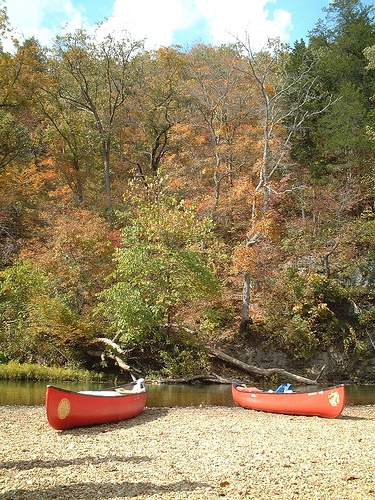
\includegraphics[width = 0.2\textwidth, height = 0.15\textheight]{canoe1}
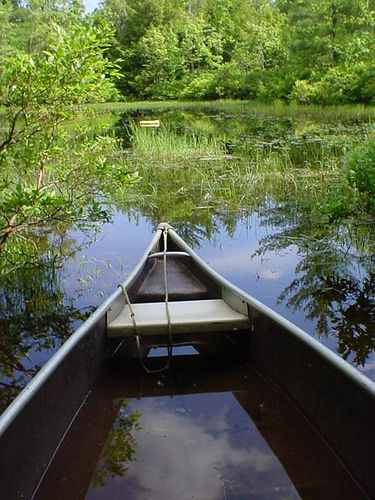
\includegraphics[width = 0.2\textwidth, height = 0.15\textheight]{canoe2}
\label{fig1:scale}
}
\subfloat[occlusion]{
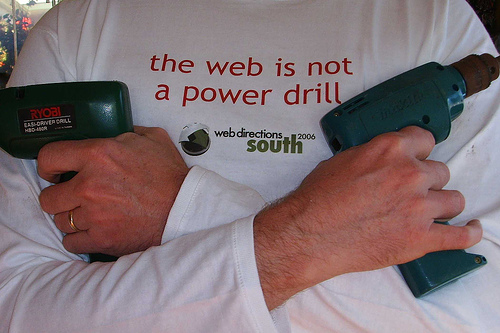
\includegraphics[width = 0.2\textwidth, height = 0.15\textheight]{pdrill1}
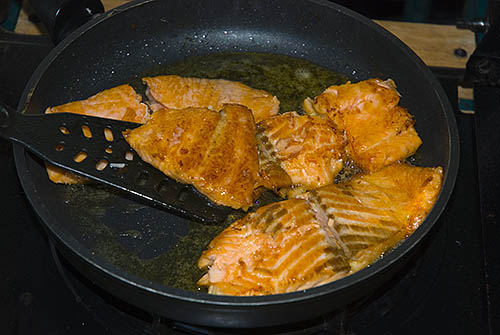
\includegraphics[width = 0.2\textwidth, height = 0.15\textheight]{spatula2}
\label{fig1:occlusion}
}
\qquad
\subfloat[pose]{
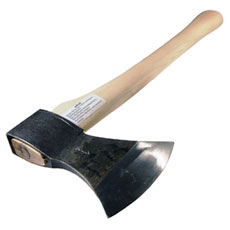
\includegraphics[width = 0.2\textwidth, height = 0.15\textheight]{hatchet1}
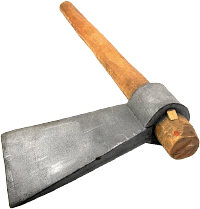
\includegraphics[width = 0.2\textwidth, height = 0.15\textheight]{hatchet2}
\label{fig1:pose}
}
\subfloat[illumination]{
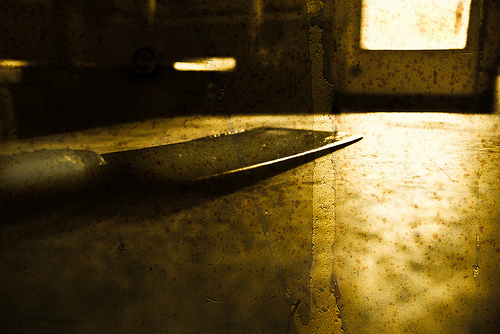
\includegraphics[width = 0.2\textwidth, height = 0.15\textheight]{cleaver2}
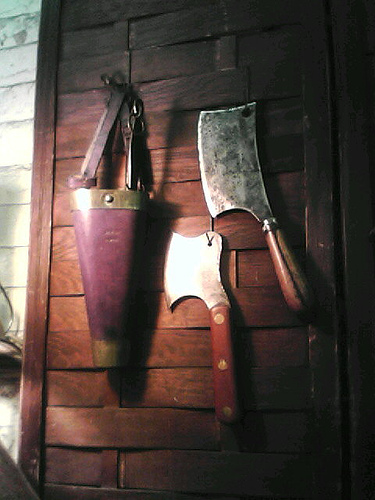
\includegraphics[width = 0.2\textwidth, height = 0.15\textheight]{cleaver3}
\label{fig1:illumination}
}
\qquad
\subfloat[clutter]{
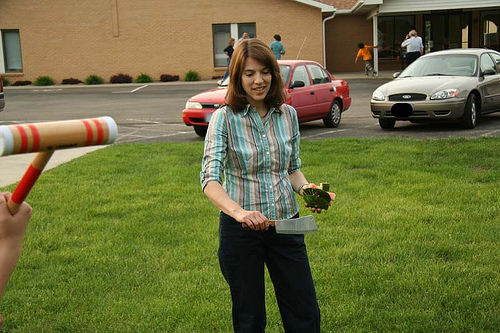
\includegraphics[width = 0.2\textwidth, height = 0.15\textheight]{cleaver1}
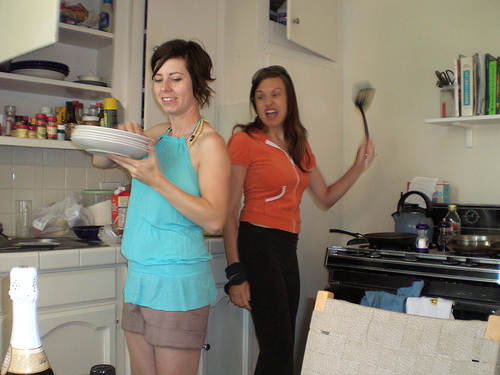
\includegraphics[width = 0.2\textwidth, height = 0.15\textheight]{spatula3}
\label{fig1:clutter}
}
\caption{Some challenges in image classification}
\end{figure}

\begin{figure}
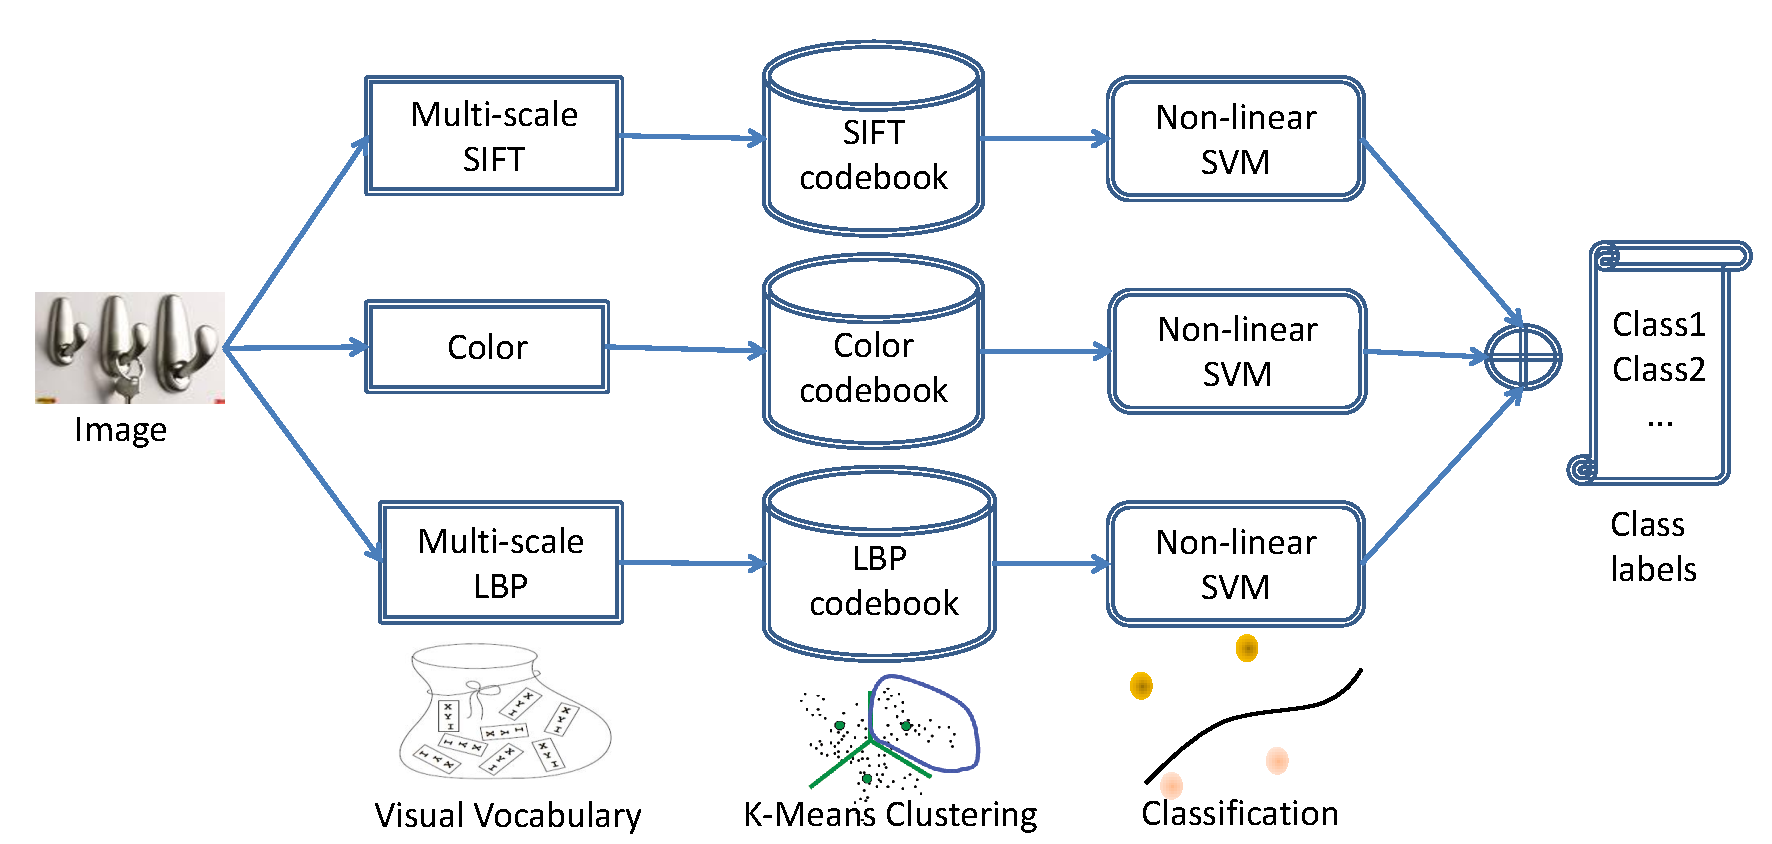
\includegraphics[width = 1\textwidth]{flowchart}
\caption{The proposed classification framework}
\end{figure}

\section{Classification Framework}
For the given classification task, we propose a three stage framework based on the Bag of Words(BOW) model. The first step comprises of densely sampling different types of features at multiple scales and generating the \textit{visual vocabulary}. This is followed by doing k-means clustering for creating the \textit{visual codebook} for each distinct feature. This is analogous to the Bag of Words (BOW) model quite popular in the information retrieval domain. Finally, non-linear support vector machines are trained on each codebook, and their prediction outputs combined to generate the class labels.

\subsection{Feature Descriptors}
It is quite vital to represent images in terms of features which can sufficiently distinguish between different classes for the purpose of image classification. In our approach we use three different types of descriptors based on the type of information they capture from an image:

\begin{itemize}

\item \textit{Scale Invariant Feature Transform (SIFT)}:

\item \textit{Local Binary Patterns (LBP)}:

\item \textit{Color}:

\end{itemize}

\begin{figure}
\centering
\subfloat[Dense feature extraction]{
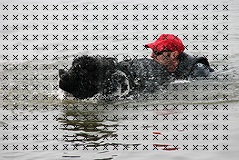
\includegraphics[width = 0.4\textwidth, height = 0.25\textheight]{dog_intdet}
\label{fig1:subfig5}
}
\subfloat[Visual codebook generation]{
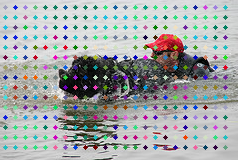
\includegraphics[width = 0.4\textwidth, height = 0.25\textheight]{dog_quantized}
}
\caption{Illustrating the dense feature extraction and the codebook generation process.}
\end{figure}


\subsection{Multi-scale dense feature extraction}


\subsection{Visual codebook generation}


\begin{figure}[H]
\centering
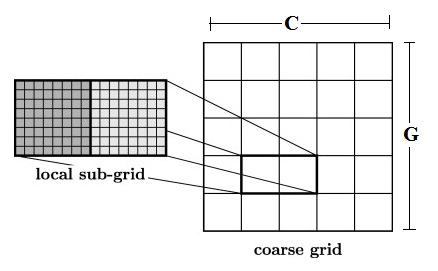
\includegraphics[width = 0.5\textwidth, height =0.2\textheight]{gridsearch}
\caption{Coarse-to-fine grid search for RBF-SVM optimum parameters}
\label{fig:gridsearch}
\end{figure}

\subsection{Classification}
The final step in the proposed paradigm involves training classifiers based on the generated visual codebooks, and then using them to predict test samples. However, there are many considerations within this step including the choice of classifiers as well the combination of classifiers.

\subsubsection{Choice of Classifiers}
We initially experimented with using the nearest neighbor classifier as well as using boosted decision stumps. The rank-5 accuracies using the SIFT codebook (5-fold cross validation on the training data) were around 66\% and 78\% respectively for these classifiers. Radial basis Support Vector Machines (RBF-SVMs) outperformed all other classifiers in our initial set of experiments and therefore we settled with using them as the base classifiers. In the proposed classification framework, three different Radial basis Support Vector Machines (RBF-SVMs) are trained for each of the three different visual codebooks.

\subsubsection{Parameter Selection}
Effectiveness of SVM classifiers depends on the selection of the right set of parameters. There are two different parameters for RBF-SVM namely the soft margin parameter $C$ and the kernel width $G$. For obtaining the optimum set of parameters, we do a coarse-to-fine grid search over the 2-dimensional space of $C$ and $G$ as shown in Figure \ref{fig:gridsearch}. Basically, this involves optimizing the 5-fold cross validation accuracies on the training set over a grid of coarse combinations of parameters $C$'s and $G$'s, and then fine tuning the parameters by doing a finer search inside the coarser grid.

\begin{figure}
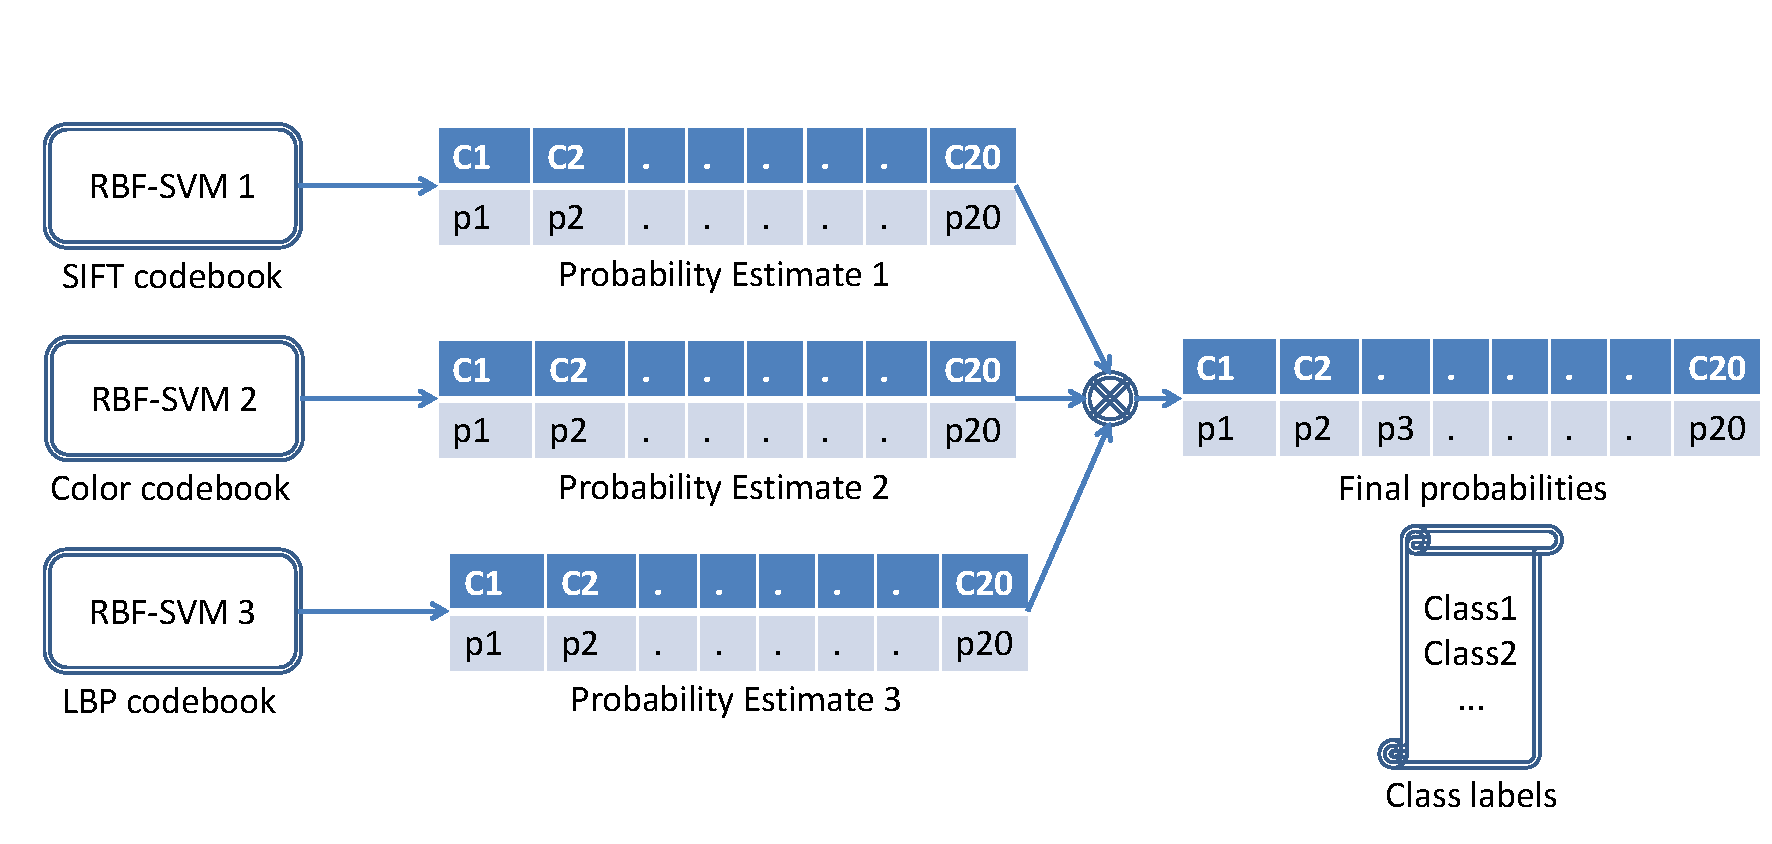
\includegraphics[width = 1\textwidth]{classifiercombination}
\caption{Classifier Combination using Product Fusion}
\label{fig:classifiercombination}
\end{figure}

\subsubsection{Classifier Combination}
Since the three non-linear SVM classifiers are trained on the three different visual codebooks corresponding to multiscale SIFT, LBP and Color features, they work on features which capture different type of information content from an image. Assuming that the classifiers are independent is a safe assumption in such a scenario. We therefore fuse the classifiers using the product fusion rule as shown in Figure \ref{fig:classifiercombination}. Each classifier independently outputs the probability of the test sample belonging to each of the different classes. The probability values corresponding to each of the classes are multiplied together to yield the final probability estimate. These estimates are then sorted in a descending order to get the top-5 class labels for the test sample.

\section{Results}
\begin{itemize}
\item Top-5 accuracy:
\begin{itemize}
\item \textbf{Training Set}: 99.99\%
\item \textbf{Validation Set}: 88.55\%
\item \textbf{Test Set}: 88.94\%
\end{itemize}
\item Classes where the approach really works well: \textit{odometer, rapeseed, website}.
\item Classes where the approach does not work very well: \textit{lopener, hatchet, cleaver}.
\end{itemize}

\begin{center}
\begin{tabular}[]{| c | c | c | }
\hline
\multicolumn{2}{|c|}{\textbf{Classification Accuracy} (\%)} \\
\hline
SIFT & 81.55\\
\hline
LBP & 82.6\\
\hline
Color & 77.58\\
\hline
SIFT + LBP & 84.6\\
\hline
SIFT + LBP + Color & \textbf{88.55}\\
\hline
\end{tabular}
\captionof{table}{Classification accuracy of the proposed approach on the validation set.}
\end{center}

\bibliographystyle{plain}
\bibliography{report}

\end{document}